%%
%% VTTSI-Chat CI/HCOMP 2026 Demo Submission
%% Demo track: non-anonymized, non-archival, 1--2 page system description.
%%
\documentclass[manuscript,screen]{acmart}

\usepackage{tabularx}
\usepackage{booktabs}

\setcopyright{none}
\settopmatter{printacmref=false, printccs=true, printfolios=true}
\renewcommand\footnotetextcopyrightpermission[1]{}
\pagestyle{plain}

\acmConference[CI/HCOMP '26]{The 14th ACM Collective Intelligence Conference
  and ACM Conference on Human-AI Complementarity and Alignment}{September
  27--30, 2026}{Near Washington, DC, USA}
\acmYear{2026}
\copyrightyear{2026}

\begin{document}

\title[VTTSI-Chat CI Demo]{VTTSI-Chat: A Human-AI Collective Intelligence Demo
for Real-Time Traffic Safety}

\author{Cheng-Shun Chuang}
\affiliation{%
  \department{Computer Science}
  \institution{Virginia Tech}
  \city{Alexandria}
  \state{Virginia}
  \country{USA}}
\email{cchengshun@vt.edu}

\author{Jason Cusati}
\affiliation{%
  \department{Computer Science}
  \institution{Virginia Tech}
  \city{Blacksburg}
  \state{Virginia}
  \country{USA}}
\email{djjay@vt.edu}

\renewcommand{\shortauthors}{Chuang and Cusati}

\begin{abstract}
VTTSI-Chat is a live human-AI traffic-safety command center that combines
connected-vehicle telemetry, crash-history analytics, a geospatial dashboard,
and a tool-grounded conversational agent. The demo shows complementarity in
practice: algorithms produce risk evidence, while human operators, planners,
and responders use SafetyChat to ask contextual questions, inspect evidence,
and decide what action is warranted. We also expose the project's
``constellized'' human-AI engineering method: multiple AI partners coordinated
through shared memory, tests, cloud checks, and human verification.
\end{abstract}

\begin{CCSXML}
<ccs2012>
 <concept>
  <concept_id>10003120.10003130.10003131</concept_id>
  <concept_desc>Human-centered computing~Interactive systems and tools</concept_desc>
  <concept_significance>500</concept_significance>
 </concept>
 <concept>
  <concept_id>10010147.10010178.10010187</concept_id>
  <concept_desc>Computing methodologies~Intelligent agents</concept_desc>
  <concept_significance>300</concept_significance>
 </concept>
 <concept>
  <concept_id>10002951.10003227.10003241</concept_id>
  <concept_desc>Information systems~Decision support systems</concept_desc>
  <concept_significance>300</concept_significance>
 </concept>
</ccs2012>
\end{CCSXML}

\ccsdesc[500]{Human-centered computing~Interactive systems and tools}
\ccsdesc[300]{Computing methodologies~Intelligent agents}
\ccsdesc[300]{Information systems~Decision support systems}

\keywords{collective intelligence, human-AI collaboration, human-AI
complementarity, traffic safety, geospatial dashboard, agentic AI, memory
systems}

\maketitle

\section{Demo Motivation}

Collective intelligence emerges when diverse participants and information
sources are coordinated into better decisions than any single participant could
produce alone. VTTSI-Chat applies this idea to urban traffic safety. The live
system connects three kinds of intelligence: (1) roadway sensors and connected
vehicles, which supply high-frequency signals; (2) statistical and
multi-criteria models, which transform those signals into interpretable risk
scores; and (3) human operators, planners, and responders, who bring local
judgment and accountability. SafetyChat adds a fourth coordinating layer: a
tool-grounded AI partner that can retrieve live scores, compare intersections,
explain causal factors, summarize trends, and run guarded read-only database
queries.

This framing aligns with the CI/HCOMP 2026 theme of \emph{Connections}: the
demo connects data streams to human decisions, connects geospatial analytics
to natural language explanation, and connects human developers to AI partners
through a documented project-memory workflow. VTTSI-Chat is not an AI
replacement for operators. It is a supervisory human-AI system: AI accelerates
retrieval and synthesis, while humans set goals, interpret uncertainty, and
make final decisions.

\section{System and Interaction}

The deployed system is available at
\url{https://safety-index-frontend-180117512369.europe-west1.run.app/}. A
Vite React dashboard communicates with a FastAPI backend on Google Cloud Run
and Cloud SQL/PostGIS. The dashboard monitors 18 geospatially registered
intersections in Falls Church, Virginia. Its operations view shows KPI cards,
an OpenStreetMap network-risk map, selected-site details, a priority queue,
and an RT--SI/MCDM blending control. Other panels support trend analysis,
crash-proximity validation, sensitivity analysis, and read-only database
exploration. SafetyChat remains visible as a persistent assistant dock.

SafetyChat uses typed backend tools instead of free-form claims:
\texttt{get\_safety\_score}, \texttt{get\_component\_breakdown},
\texttt{get\_historical\_baseline}, \texttt{compare\_intersections},
\texttt{get\_trend\_data}, and a guarded \texttt{run\_sql\_query}. The SQL
tool rejects comments, multiple statements, and write/DDL keywords; local
database paths use SQLAlchemy statements where available. Frequently called
read endpoints use per-instance caching, and local plus cloud tests verify
the map, chat tools, SQL guardrails, and production API behavior.

\begin{figure}[t]
\centering
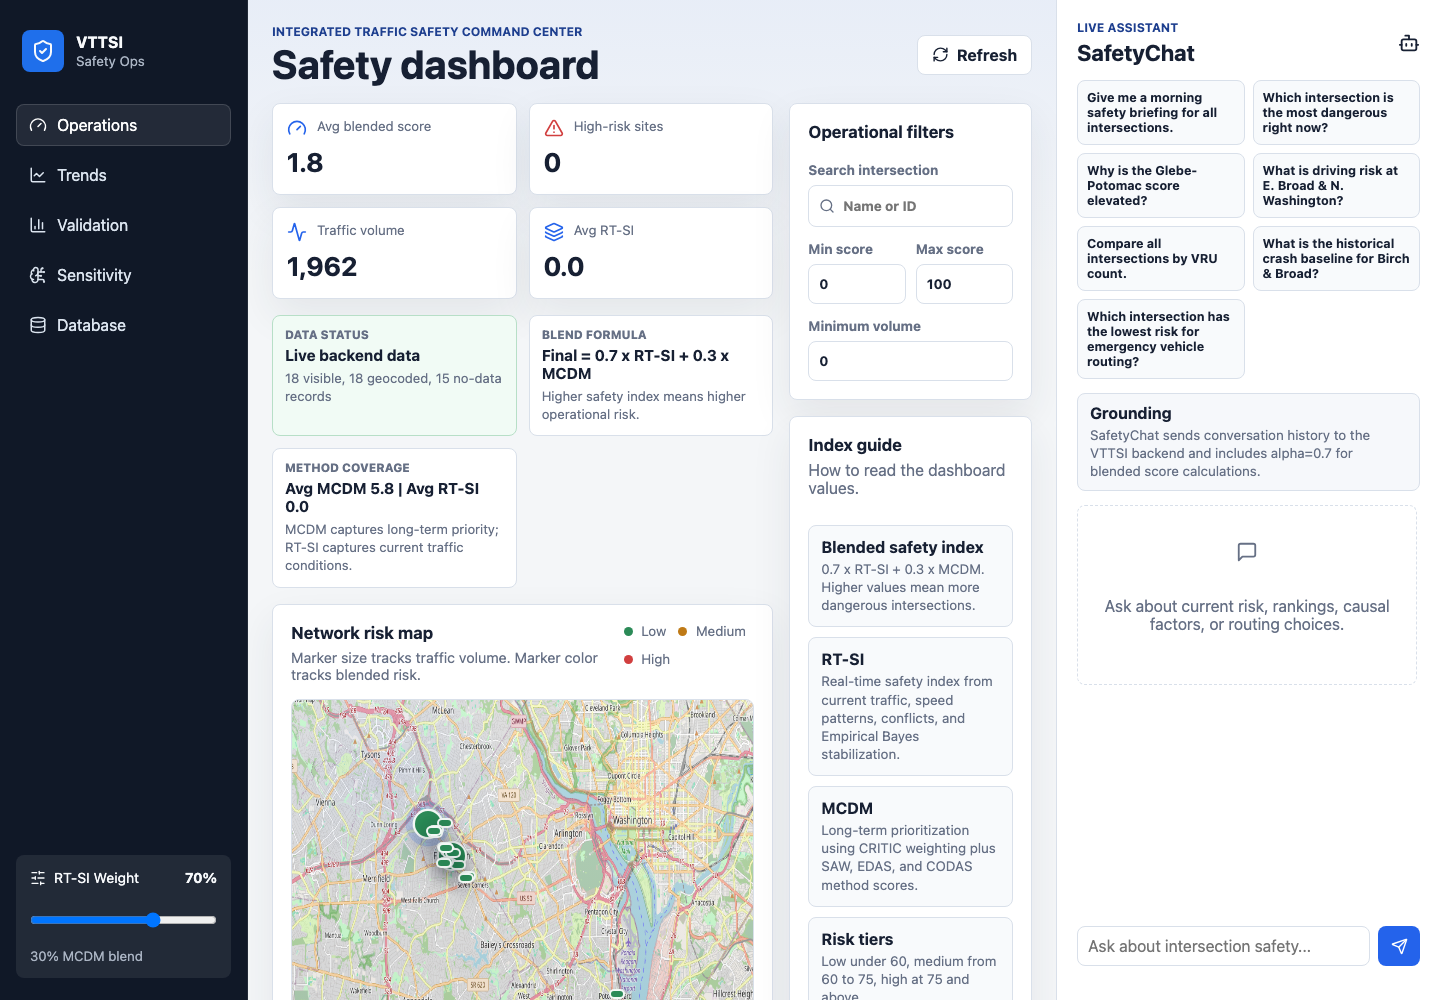
\includegraphics[width=.48\textwidth]{vite-dashboard-chat.png}\hfill
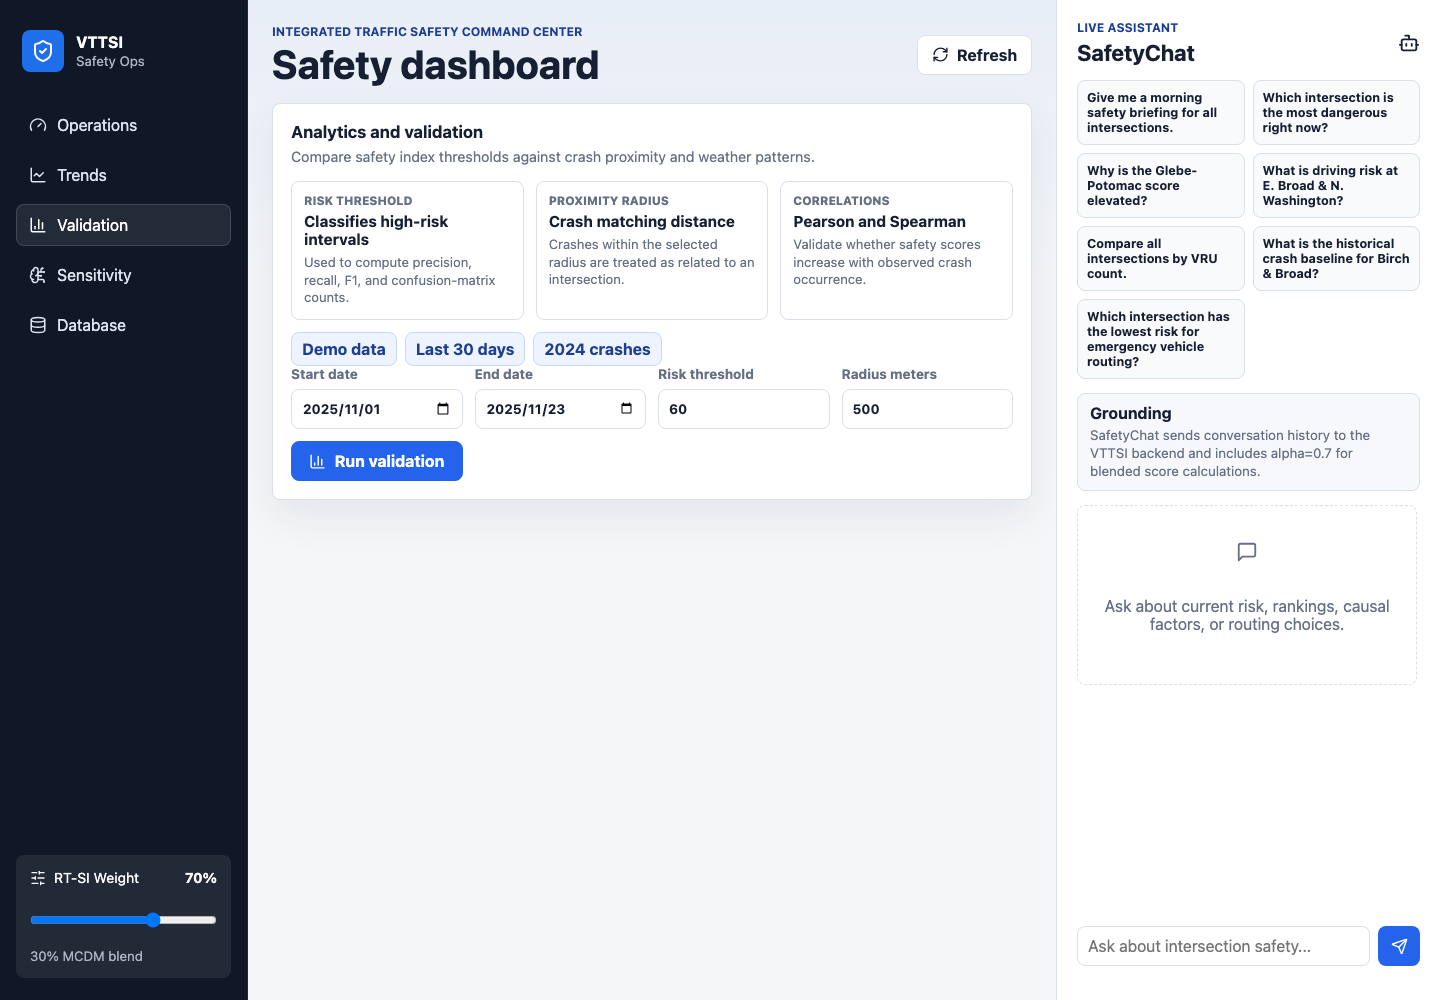
\includegraphics[width=.48\textwidth,trim=250 405 380 0,clip]{vite-validation.png}
\caption{Demo overview: the integrated dashboard with SafetyChat and the
crash-proximity validation workflow.}
\Description{A two-panel figure. The first panel shows the dashboard with KPI
cards, a network-risk map, controls, and the SafetyChat assistant. The second
panel shows validation controls for comparing safety-index thresholds with
crash proximity.}
\end{figure}

Attendees will try four interactions: inspect the map and adjust the
RT--SI/MCDM blend; ask SafetyChat questions such as ``Which intersection is
most dangerous right now?''; run crash-proximity validation to discuss trust
and uncertainty; and inspect the memory-bank artifacts and test logs that show
how human developers coordinated AI partners across implementation, review,
deployment, and documentation.

\section{Constellized Human-AI Engineering}

The demo is also a case study in building software with AI partners. We call
the method \emph{constellized} because different AI roles are arranged around
a persistent project memory rather than treated as a single opaque assistant.
AI partners helped with frontend migration, backend hardening, cache design,
SQL-safety regression tests, cloud endpoint tests, documentation cleanup, and
manuscript drafting. Human developers remained responsible for problem
framing, acceptance decisions, security tradeoffs, cloud operations, and final
verification.

The memory bank makes this collaboration inspectable. It records the current
system state, architectural decisions, operational constraints, troubleshooting
notes, and verification commands. Each AI-assisted change is anchored to tests,
screenshots, deployment checks, or Cloud Run/Cloud SQL state. This creates a
governance loop for human-AI software work: remember the project state,
propose changes, execute through tools, verify with tests and live endpoints,
then update memory. The demo therefore shows how collective intelligence
systems can be built both \emph{for} and \emph{through} accountable human-AI
collaboration.

\section{Logistics and Disclosure}

The demo requires one table, power, Wi-Fi, and a laptop browser. A video
walkthrough will accompany the EasyChair submission. Generative AI tools,
including OpenAI ChatGPT, Codex, and Anthropic Claude, were used as AI
partners for coding assistance, debugging, test design, documentation,
manuscript drafting, and grammar editing. The authors reviewed, verified, and
edited all AI-assisted content; the research framing, system design decisions,
claims, and final submission remain the responsibility of the authors.

\end{document}
